
\documentclass{article} 
\usepackage{french,epsfig,comment}
\usepackage[latin1]{inputenc}      

\newenvironment{solution}{\nopagebreak\par\vspace*{2mm}\underline{Solution~:}\em\par}{\par\vspace*{2mm}}


%\newtheorem{defin}{D�finition}[section]
%\newtheorem{exampl}{Exemple}[section]
%\def\Semijoin{\mathbin{\rhd\hbox to -.45em{}<}}
\def\picwidth{16cm}


%\includecomment{solution}


\begin{document}

\begin{center}
\Large\bf Syst�mes de Gestion de Bases de Donn�es ICPJ B6/B7\\ \ \\
\Large\bf EXAMEN\\ \ \\
\large\bf Jeudi 22 Juin 2000
\end{center}

%%%%%%%%%%%%%%%%%%%%%%%%%%%%%%%%%%%%%%%%%%%%%%%%%%%%%%%%%%%%

\section{Indexation (? points)}

\subsection*{Index dense et non-dense}

Soit un fichier tel que 
chaque page peut contenir 10 articles. On indexe
ce fichier avec un niveau d'index, et on suppose
qu'une page d'index contient 100 paires (cl�, pointeur).

Si $n$ est le nombre
d'articles, donnez la fonction de $n$
permettant d'obtenir  le nombre minimum de pages pour
les structures suivantes\,: 
\begin{enumerate}
  \item Un fichier avec un index dense.
  \item Un fichier tri� sur la cl� avec un index non-dense.
\end{enumerate}

\begin{solution}
(1) $n/10$ et $n/100$, soit $\frac{11 \times n}{100}$ pages.
(2) Il faut seulement $n/10$ paires (cl�, pointeur),
donc $n/1000$ pages, pour un total  de $\frac{101\times  n}{1000}$ pages.

\end{solution}


\subsection*{Arbre-B}

On reprend les hypoth�ses pr�c�dentes, et on indexe
maintenant le fichier avec un arbre-B+. Les feuilles de l'arbre 
contiennent donc des pointeurs vers le fichier, et les noeuds internes
des pointeurs vers d'autres noeuds (voir figure~\ref{icpj}). 
On suppose qu'une page
d'arbre B+ est pleine � 70\,\% (69 cl�s, 70 pointeurs). 

\begin{enumerate}
  \item Le fichier est tri� sur la cl�, et index�
     par un arbre-B+  dense.  Donnez (1) le nombre
de niveaux de l'arbre pour un fichier de 1~000~000 articles, (2) le nombre de
pages utilis�es (y compris l'index), et (3) le nombre 
d'acc�s disque pour rechercher un article par sa cl�.


\begin{solution}
Il y a 100~000 pages de donn�es. Un million
d'articles, donc $\frac{1M}{70} = 14~286$ pages pour le dernier
niveau de l'arbre B+. On divise encore par 70\,:
204 pages au niveau $l-1$, 3 pages au niveau sup�rieur, et 1 page
 pour la racine.

Il faut donc lire 4+1 pages pour acc�der � un article
par sa cl�.
\end{solution}
%  \item Idem que pr�c�demment, mais le fichier n'est pas tri�.


  \item On effectue maintenant une recherche par intervalle
      ramenant 1~000 articles.  D�crivez
    la recherche et donnez le nombre d'acc�s
      disque dans le pire des cas.
\begin{solution}
Recherche sur le plus petit �l�ment (4 pages), puis lecture de 
$\frac{1000}{70} = 14$ pages
en suivant le niveau des feuilles de l'arbre B+. Pour chaque pointeur 
vers un objet il faut lire une page dans le pire des cas, soit
1~000 pages. Total\,: 1018 pages.
\end{solution}

  \item M�mes questions que (1), mais l'arbre-B+ est non dense.
\begin{solution}
Il faut indexer 100~000 pages. Donc 1429 pages au dernier niveau, 
puis 20, puis 1. On �conomise un niveau.
\end{solution}

\end{enumerate}

\subsection*{Op�rations sur arbre B+}

Soit l'arbre B+ de la figure~\ref{icpj}. Expliquez
les op�rations suivantes, et donnez le nombre
d'acc�s  n�cessaire {\em aux pages de l'arbre B+} (ne tenez pas compte
de l'acc�s au fichier).

\begin{enumerate}
  \item Recherche de l'article 41.
  \item Recherche des articles 20 � 30.
  \item Insertion des artilces 1 et 4.
  \item Destruction de l'article 23.
\end{enumerate}

\begin{figure}
    \centerline{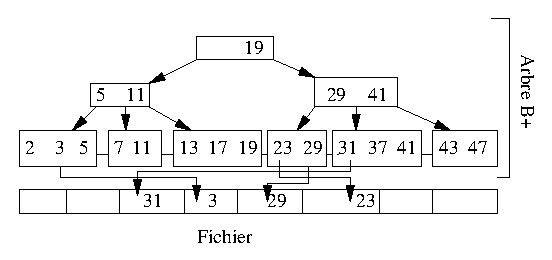
\psfig{figure=icpj.eps}}  
    \caption{Un arbre B+}  
    \label{icpj}  
\end{figure}
%%%%%%%%%%%%%%%%%%%%%%%%%%%%%%%%%%%%%%%%%%%%%%%%%%%%%%%%%%%%


\section{Concurrence et reprise sur pannes (? points)}

Soit les histoires suivantes\,:

\begin{enumerate}
  \item $r_1(A) r_2(A) r_3(B) w_1 (A) r_2(C) r_2(B) w_2(B) w_1(C) C_1 C_2$ 
  \item $r_1(A) w_1(B) r_2(B) C_1 w_2(C) C_2 r_3(C) w_3(A) C_3$
  \item $r_1(A) r_2(A) w_1(B) w_2(B) r_1(B) r_2(B) w_2(C) w_1(D) C_1 C_2$
\end{enumerate}

\begin{itemize}
  \item Lesquelles sont s�rialisables\, (donnez le graphe de s�rialisabilit�
pour chacune).
\begin{solution}
(1) Oui. $T3 \to T2 \to T1$\\
(2) Oui.  $T1 \to T2;  T2 \to T3; T1 \to T3$\\
(3) Non. $T1 \to T2 ; T2 \to T1$
\end{solution}

  \item Appliquez un verrouillage � deux phases � celles
   qui ne sont pas s�rialisables.

\end{itemize}

\end{document}
